\chapter{Objectif du Projet}
\paragraph{}
Le but de ce projet est de pouvoir extraire un automate à partir du code source Java d’une applet JavaCard et le comparer à un automate de référence. Dans cette partie, afin d'expliquer au mieux les enjeux et les besoins nous commenceront par expliquer l'intérêt de l'extraction d'automate pour une application sous JavaCard, puis nous donnerons un court exemple de ce qui sera demandé à l'application.

\section{Intérêt de l'extraction d'automates à partir de code source}



\paragraph{Un objectif de sécurité}En effet, une application pour une carte à puce est souvent liée à un domaine en rapport à la sécurité (passeport de sécurité par exemple), à la banque (carte bancaire) ou bien encore à la téléphonie (carte SIM). Tout ces domaines d'application sont liés intimement à des données pouvant être très sensibles ou à garder à la seule connaissance de l'utilisateur légitime.

Exporter une application sous forme de graphe permet de vérifier la présence éventuelle de faille de sécurité.

\paragraph{Une autre utilisation possible}Comme nous l'avons dit ci-dessus, un tel outil peut être employé à la sécurisation de code et ainsi aider le développeur à générer une application la plus solide possible. Un autre aspect peut être celui de l'attaque. Il est tout à fait raisonné de penser qu'entre les mains d'experts, ce genre d'outil peut aider les chercheurs à trouver de nouvelles failles et ainsi les révéler pour les corriger.


\section{Mise en pratique sur une applet simple}

\paragraph{}
Tout d’abord il est nécessaire de décrire les différents états de l’applet ainsi que les transitions entre les états qui correspondent à la réception d’une commande \gls{APDU}. Nous devons repérer dans le code les réceptions de commande \gls{APDU}, déterminer les valeurs qu’elles peuvent prendre et créer l’arbre des contraintes de l’applet.
\paragraph{}
Ensuite nous pouvons construire un automate montrant les états et les commandes \gls{APDU} à envoyer pour passer de l’un à l’autre. Il sera alors possible de le comparer à l’automate de spécification de l’applet.

\paragraph{}
Le programme suivant est la partie métier d’un applet simplifiée de gestion bancaire. Cet applet propose deux fonctionnalités : consulter son solde avec le code 0x34 ou retirer de l’argent avec le code 0x38. Une protection basique est en place pour empêcher l’utilisateur de retirer plus d’argent que son compte n’en possède.

\textit{Note~:} Le tableau \verb|buffer| contient l'\gls{APDU}.

\begin{minted}[fontsize=\footnotesize]{java}
public void process(APDU apdu) throws ISOException {
  byte[] buffer = apdu.getBuffer();
      
  if(buffer[ISO7816.OFFSET_CLA] != (byte) 0x80)
    ISOException.throwIt(ISO7816.SW_CLA_NOT_SUPPORTED);
      
  short octetsLus;
      
  switch(buffer[ISO7816.OFFSET_INS]){
  case (byte) 0x34:
      octetsLus = apdu.setIncomingAndReceive();
      if(octetsLus != (short) 0)
	ISOException.throwIt(ISO7816.SW_WRONG_LENGTH);
      if(buffer[ISO7816.OFFSET_P1] != (byte) 0x00 
	  && buffer[ISO7816.OFFSET_P2] != (byte) 0x00 )
	ISOException.throwIt(ISO7816.SW_INCORRECT_P1P2);
      Util.setShort(buffer, (short) 0, balance);
      apdu.setOutgoingAndSend((short)0 , (short)2);
      return;
    case (byte) 0x38:
      octetsLus = apdu.setIncomingAndReceive();
      if(octetsLus != (short)2)
	ISOException.throwIt(ISO7816.SW_WRONG_LENGTH);
      if(buffer[ISO7816.OFFSET_P1] != (byte)0x00 
	  && buffer[ISO7816.OFFSET_P2] != (byte)0x00)
	ISOException.throwIt(ISO7816.SW_INCORRECT_P1P2);
      short delMont = Util.getShort(buffer, (short)5);
      if(balance < delMont)
	ISOException.throwIt(ISO7816.SW_COMMAND_NOT_ALLOWED);
      balance -= delMont;
      return;
  default:
      ISOException.throwIt(ISO7816.SW_INS_NOT_SUPPORTED);
  }

}
\end{minted}

Une fois l'application analysée par le programme d'analyse concolique, on souhaite obtenir un graphe de la forme : 

~

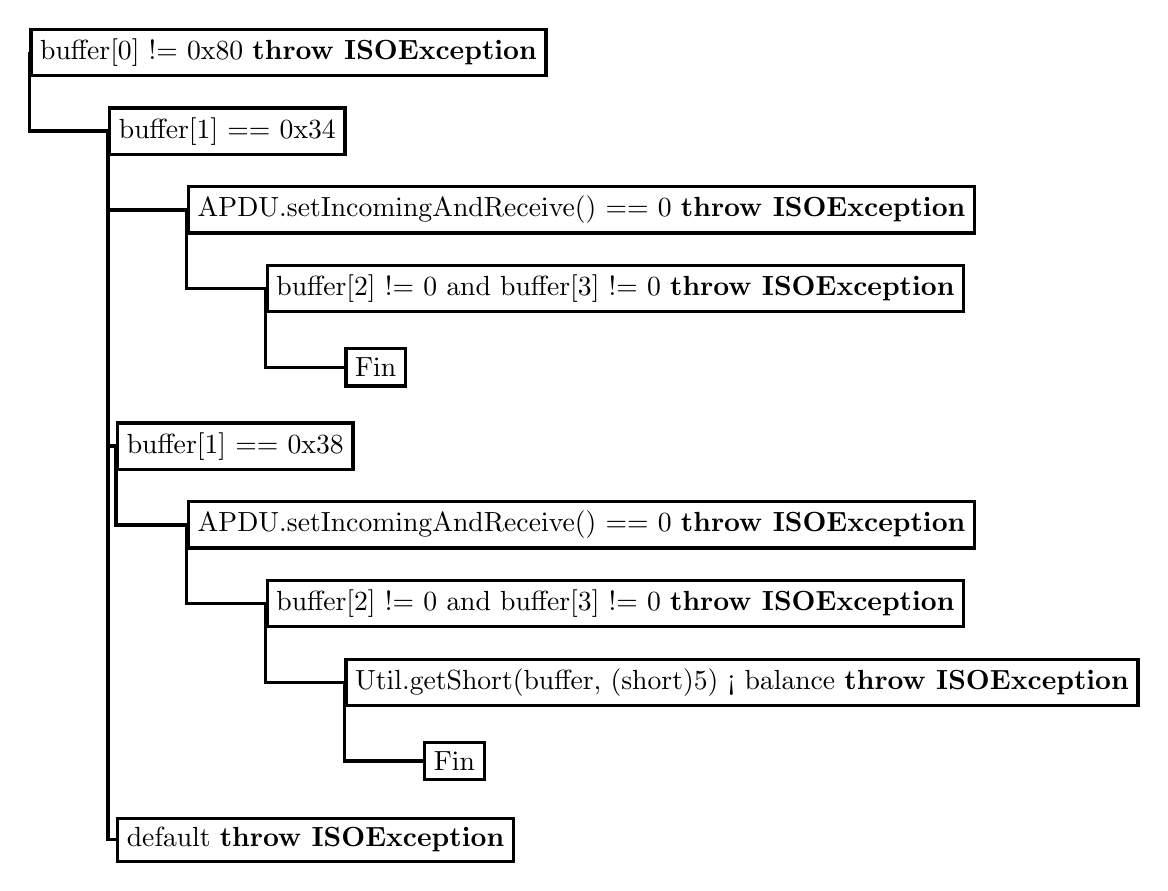
\begin{tikzpicture}[very thick,top color=white,bottom color=gray]
\node[anchor=west,draw] (A) at (0,0) {buffer[0] != 0x80 \textbf{throw ISOException}};
\node[anchor=west,draw] (B) at (1,-1) {buffer[1] == 0x34};
\node[anchor=west,draw] (C) at (2,-2) {APDU.setIncomingAndReceive() == 0 \textbf{throw ISOException}};
\node[anchor=west,draw] (D) at (3,-3) {buffer[2] != 0 and buffer[3] != 0 \textbf{throw ISOException}};
\node[anchor=west,draw] (E) at (4,-4) {Fin};
\node[anchor=west,draw] (F) at (1.1,-5) {buffer[1] == 0x38};
\node[anchor=west,draw] (G) at (2,-6) {APDU.setIncomingAndReceive() == 0 \textbf{throw ISOException}};
\node[anchor=west,draw] (H) at (3,-7) {buffer[2] != 0 and buffer[3] != 0 \textbf{throw ISOException}};
\node[anchor=west,draw] (I) at (4,-8) {Util.getShort(buffer, (short)5) < balance \textbf{throw ISOException}};
\node[anchor=west,draw] (J) at (5,-9) {Fin};
\node[anchor=west,draw] (K) at (1.1,-10) {default \textbf{throw ISOException}};


\draw (A.west) |- (B.west);
\draw (B.west) |- (C.west);
\draw (C.west) |- (D.west);
\draw (D.west) |- (E.west);
\draw (B.west) |- (F.west);
\draw (F.west) |- (G.west);
\draw (G.west) |- (H.west);
\draw (H.west) |- (I.west);
\draw (I.west) |- (J.west);
\draw (B.west) |- (K.west);

\end{tikzpicture}

\paragraph{}
Une fois le graphe extrait, nous souhaitons créer un automate représentant le fonctionnement de l'application, en voici un exemple en lien avec le graphe précédent :
